\documentclass[tikz,border=10pt]{standalone}
\usetikzlibrary{calc}
\begin{document}
% Scale: s = 0.015873 cm/px, origin at V, y flipped
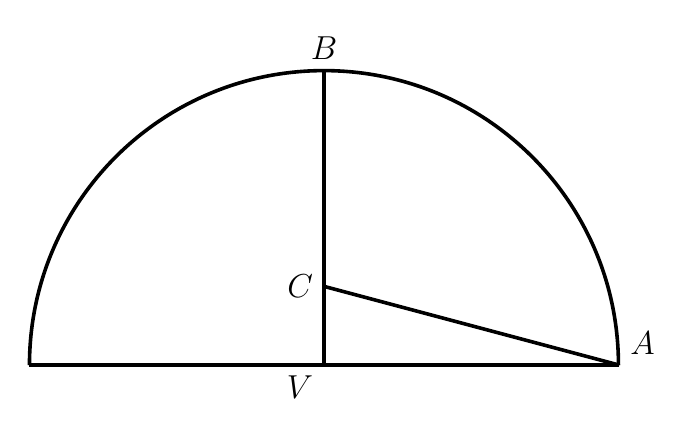
\begin{tikzpicture}[line width=1.3pt, line join=round, lbl/.style={font=\fontsize{13}{15.6}\selectfont}]
  % Named coordinates (cm)
  \coordinate (V) at (0,0);
  \coordinate (D) at (-3.74,0);
  \coordinate (A) at (3.75,0);
  \coordinate (B) at (0,3.74);
  \coordinate (C) at (0,1.00);

  % Upper semicircle, centre V, radius 3.74 cm (180 -> 0 degrees through B)
  \draw (D) arc[start angle=180, end angle=0, radius=3.74];

  % Diameter DA (solid)
  \draw (D) -- (A);

  % Segment BV (solid); stops at B rather than overshooting it
  \draw (B) -- (V);

  % Segment AC (solid)
  \draw (A) -- (C);

  % Labels (math mode, 13 pt on 15.6 pt leading)
  \node[lbl, above] at (B) {$B$};
  \node[lbl, left]  at (C) {$C$};
  \node[lbl, above right] at (A) {$A$};
  \node[lbl, below left]  at (V) {$V$};
\end{tikzpicture}
\end{document}